% $Id: chapter9.tex 1790 2010-09-28 16:46:40Z jabriffa $
\chapter {The Algorithm}

\section{Planning}

Most ranking algorithms as have been discussed, mainly revolve around some combination of voting and time. While some have more complicated parameters, they are usually tailored to the website's philosophy, such as the use of  the penalty attribute in Hacker Rank. However, since this project aims to provide the user with an automated display of the most relevant news tailored to the user's interests, voting will be replaced with the user's interests.
\paragraph{}
The user should be able to select interests in their account page, which have a score associated with them and that score should be a significant contributor in the score of a post. When a post gets created is also be a valuable attribute, and it should be beneficial to the algorithm since time can never be the same even if the rest of the attributes are the same, differentiating in that way two potentially similar posts. Another vital aspect to consider is how many interests does the post have, in which the user is not interested. However, the impact of this attribute should not be as negatively equal to a relevant interest in a post. For example, if the score of the common interest between user and post is equal to 10, a non-common interest should impact the overall score by -5 or lower. Lastly, the concept of banning or negatively reducing a ranking score is an essential attribute and can be detrimental in the image and environment that a system portrays.

\section {Designing}

\paragraph{}

After a couple of failed attempts, the final algorithm was a combination time, common interests, non-common interests and penalties. The algorithm relies on multiplication and division to increase or decrease a rating for the sake of simplicity bundled with the fact that time which when denoted in timestamps usually tends to be a couple of digits long in the first place. The algorithm can be seen below:

\begin{figure}[htbp]
\begin{minipage}[t]{\linewidth}
  \centering
    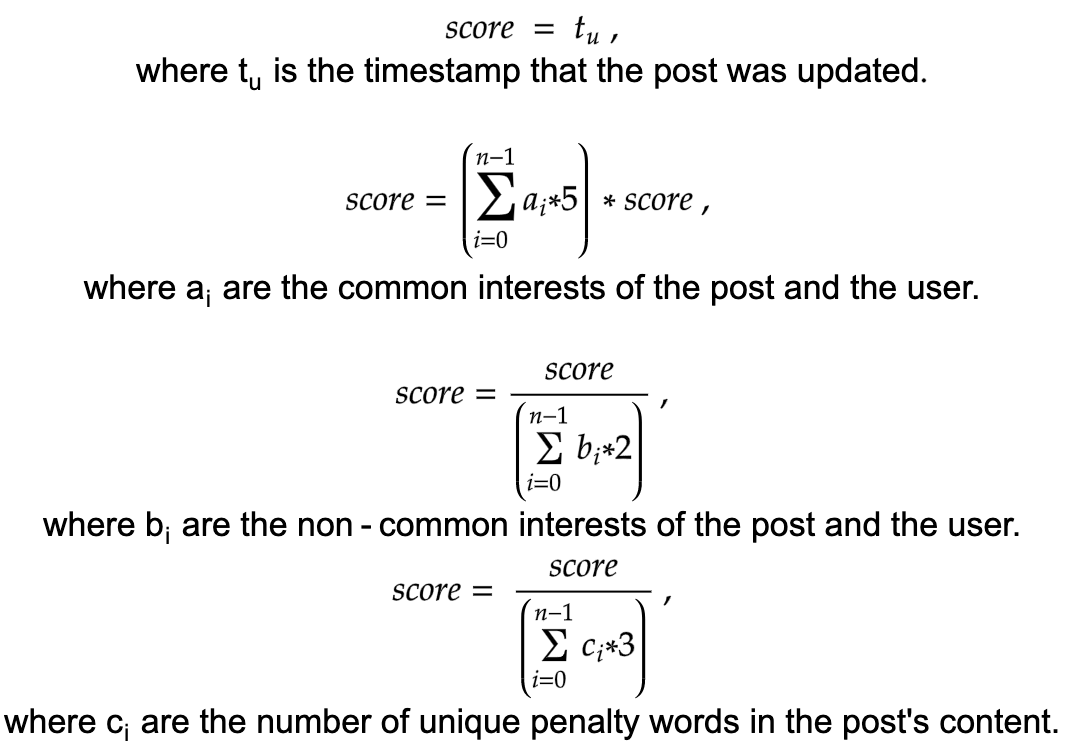
\includegraphics[scale=0.4]{Figures/algorithm}
    \caption{The stages of the final ranking algorithm.}
    \label{fig:algorithm}
\end{minipage}%
\end{figure}

% \begin{figure}
%   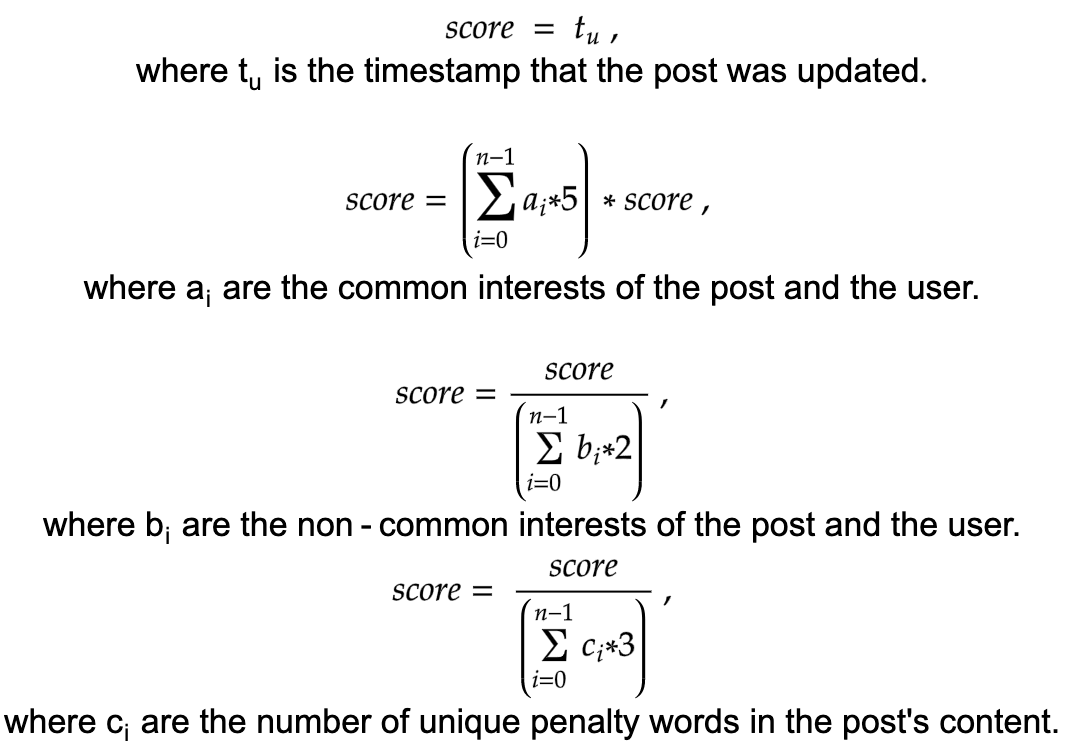
\includegraphics[scale=0.4]{Figures/algorithm}
%   \caption{The stages of the final ranking algorithm.}
%   \label{fig:algorithm}
% \end{figure}

Since time was going to be used as timestamps which usually tend to be a couple of digits long, I decided to use multiplication and division to increase or decrease a rating was used. As portrayed in ~\ref{fig:algorithm}, if the user is not logged in or, they have no interest selected, the score of each post is set equal to the time that the post was updated. However, if the user is logged in and has selected interests, then the existing score is multiplied by 5 for each common interest of the user and the post.

For the deduction part of the algorithm, the score is halved for each non-common interest. This decision makes sense since, if a potential user is interested in news, a post with only the "news" interest will rank higher than a post with the news and music interest unless the first post is much older than the second one. The last deduction part of the algorithm is penalties. Penalties, that at the moment are profanity words, essentially counter a common interest, since the score of a post is divided by 5 for each penalized word the post contains.

\section {Creating}

Assigning each post with a score based on the parameters aforementioned happens when the "get\_blog\_queryset" function is called in "home\_screen\_view", and the code featured below explains is part of the "get\_blog\_queryset" function.


\lstset{language=Python}
\lstset{frame=lines}
\begin{lstlisting}
# Checks if the user is authenticated.
if user.is_authenticated: #1
  pen_post = [] #1

  for penalty in penalty_list: #n
    penalized_posts = BlogPost.objects.filter(
    Q(title__contains=penalty)|
    Q(body__icontains=penalty)) #n
    for q in queryset: #n
      if q in penalized_posts:
        q.bad_words = q.bad_words + 1

  for q in queryset:#n
    # A list of common interests.
    common_result = []#1
    # A list of non-common interests.
    non_common_result = []#1
    # Set's the score to the time a post is updated.
    q.post_score = q.date_updated.timestamp() #1

    for element in q.interests: #n
      # Updates based on common interests.
      if element in user.interests: #1
        common_result.append(element) #1
        q.post_score = q.post_score * (len(common_result) * 5) #1

      # Updates based on non-common interests.
      if element not in user.interests: #1
        non_common_result.append(element) #1
        q.post_score = q.post_score / (len(non_common_result) * 2) #1

    # Updates based on penalty words.
    for post in pen_post: #n
      q.post_score = q.post_score / (q.bad_words * 5)#1
\end{lstlisting}

\section{Complexity}

The time complexity of this algorithm will be calculated with the popular big O notation. Big O notation is used in Computer Science to describe the performance or complexity of an algorithm. Big O specifically describes the worst-case scenario, and can be used to describe the execution time required or the space used (e.g. in memory or on disk) by an algorithm \cite{bell_2009_a}.

In the code listed in the above section, I have included the running complexity after each line. That way we can calculate that the worst-case complexity will never be more than $O(n^2)$.
